%Dokumentklasse

%draft als optionohne bilder für bessere performance
%\documentclass[a4paper,12pt,]{scrreprt}

%normal mit Bildern
\documentclass[
a4paper,
12pt,
draft=false]
{scrartcl}

%angepasster \today Command
\newcommand{\leadingzero}[1]{\ifnum #1<10 0\the#1\else\the#1\fi}
\newcommand{\todayDE}{\leadingzero{\day}.\leadingzero{\month}.\the\year}

%Tippbox
\newcommand{\tipp}[2]{{
		\textit{#1:}\\
		\vspace*{-5mm}
		\fbox{\parbox{\linewidth}{#2}}}}
	
%Uhr
	\newcommand{\uhr}[2]{#1:#2 Uhr}

%Bild
\newcommand{\bild}[3]{
	\begin{figure}[h!]
		\centering
		\includegraphics[width=#3\textwidth]{img/#2}
		\caption{#1}
		\label{fig:#2}
	\end{figure}
\FloatBarrier
\vspace*{-10mm}
}

%Bild in MInipage
\newcommand{\minibild}[3]{
	%\vspace{#3}
	\centering
	\includegraphics[width=#3\textwidth]{img/#2}
	\caption{#1}
	\label{fig:#2}
}

%Anmerkung
\newcommand{\anmerkung}[1]{
	\textcolor{red}{#1}
}
%\usepackage[allfiguresdraft]{draftfigure}

%Section als Chapter
\RedeclareSectionCommand[%
%beforeskip = -1sp plus -1sp minus -1sp,% kleinster negativer Wert, um den Absatzeinzug nach der Überschrift zu verhindern.
afterskip = 1.5 \baselineskip plus -1sp minus 1sp,
font = \Huge,
]{section}

\usepackage[left= 3cm,right = 2.5cm, bottom = 3cm,top = 2.5cm]{geometry}
%\usepackage[onehalfspacing]{setspace}

% ============= Packages =============
% Dokumentinformationen
\usepackage[
pdftitle={Praktikum - Umwelttechnik},
pdfsubject={},
pdfauthor={Roman-Luca Zank},
pdfkeywords={},	
%Links nicht einrahmen
hidelinks
]{hyperref}

%nur Text zum prüfen des Umfangs

% Standard Packages
%\usepackage[bottom]{footmisc}
\usepackage[utf8]{inputenc}
\usepackage[ngerman]{babel}
\usepackage{makecell}

\usepackage[T1]{fontenc}
%\usepackage{helvet}

%\renewcommand{\familydefault}{\sfdefault}

\usepackage{colortbl}
\usepackage{graphicx}
\graphicspath{{img/}}
\usepackage{mhchem}
\usepackage{fancyhdr}
\usepackage{lmodern}
\usepackage[table]{xcolor}
\usepackage{placeins}
\usepackage{booktabs}
\usepackage{caption}
\usepackage[list=true]{subcaption}
\usepackage{longtable}
\usepackage{tikz}
\usepackage{pgfplots}
\pgfplotsset{/pgf/number format/use comma}
\pgfplotsset{grid style={white!90!black}}
\usepackage{lastpage}
%\usepackage{ulem}
\usepackage{mathtools}
\usepackage{adjustbox}
\usetikzlibrary{patterns}
\usepackage{pdfpages}
\usepackage[shortlabels]{enumitem}
\usepackage{chemfig}

%Einheitenpackage
\usepackage{siunitx}  
\sisetup{	locale = DE, 
	per-mode=fraction,
	inter-unit-product=\ensuremath{\cdot},
	detect-weight = true,
	quotient-mode=fraction
}
%neue Einheiten definieren
\DeclareSIUnit\xyz{xyz}	
\DeclareSIUnit\rpm{rpm}	
\DeclareSIUnit\mws{mWS}	
\DeclareSIUnit\degrees{^\circ}
\DeclareSIUnit\kmeter{\raiseto{3}\meter}	


%Automatisch cdot statt *
\DeclareMathSymbol{*}{\mathbin}{symbols}{"01}


%Tabelle
\usepackage{tabularx}
\usepackage{tabulary}

%nur letzte Zeile der Gleichung nummerieren
\makeatletter
\def\Let@{\def\\{\notag\math@cr}}
\makeatother

% zusätzliche Schriftzeichen der American Mathematical Society
\usepackage{amsfonts}
\usepackage{amsmath}

%Abkürzungsverzeichnis
\usepackage{acronym}

%kein Abstand bei neuem Kapitel vom Seitenanfang
%\vspace*{2.3\baselineskip} = ORIGINAL
%\renewcommand*{\chapterheadstartvskip}{\vspace*{.0\baselineskip}}

%nicht einrücken nach Absatz
\setlength{\parindent}{0pt}


\urlstyle{same}

% ============= Kopf- und Fußzeile =============
\pagestyle{fancy}
%
\lhead{}
\chead{}
\rhead{}%\slshape }%\leftmark}
%%
\lfoot{}
\cfoot{}
\rfoot[{\thepage\ of \pageref*{LastPage}}]{Seite \thepage\ von \pageref*{LastPage}}
%%
\renewcommand{\headrulewidth}{0pt}
\renewcommand{\footrulewidth}{0pt}
%\renewcommand{\chapterpagestyle}{fancy}

%Fußnotelinie
%\let\footnoterule

%Fußnote mit Klammer
\renewcommand*{\thefootnote}{(\arabic{footnote})}

%Abb. statt Abbildung
\addto\captionsngerman{%
	\renewcommand{\figurename}{Abb.}%
	\renewcommand{\tablename}{Tab.}%
}

% ============= Package Einstellungen & Sonstiges ============= 
%Besondere Trennungen
%\hyphenation{De-zi-mal-tren-nung}
\usepackage[none]{hyphenat}
\hyphenpenalty=5000
\tolerance=5000
\providecommand\phantomsection{}

\usepackage{mathtools}


% ============= Dokumentbeginn =============

\begin{document}
%Seiten ohne Kopf- und Fußzeile sowie Seitenzahl
\pagestyle{empty}

%\begin{center}
\begin{tabular}{p{\textwidth}}


\begin{center}

\includegraphics[scale=0.75]{logos.jpg}\\
\end{center}


\\

\begin{center}
\LARGE{\textsc{
Protokoll \\
Instrumentelle Analytik\\
}}
\end{center}

\\

%\begin{center}
%\large{Fakultät für Muster und Beispiele \\
%der Hochschule Musterhausen \\}
%\end{center}
%
%\\

\begin{center}
\textbf{\Large{Versuch 3.2}}
\textbf{\Large{Gasprobennahme von Raumluft und Ermittlung der \ce{NO2}-Konzentration}}
\end{center}


\\

\begin{center}
\Large{\textbf{Teilnehmer:}} \\ 
\end{center}
\begin{center}
\large{Willy Messerschmidt} \\
\large{Roman-Luca Zank} \\
\end{center}


\\ \\ \\ \\

\begin{center}
\begin{tabular}{lll}
\large{\textbf{Protokollführer:}} & & \large{Roman-Luca Zank}\\
&&\\
\large{\textbf{Datum der Versuchsdurchführung:}}&& \large{27.05.2021}\\
&&\\
\large{\textbf{Erstabgabe:}}&& \large{\todayDE}\\
\end{tabular}
\end{center}

\\ \\ \\ \\ \\ \\ 

\large{Merseburg den \todayDE}

\end{tabular}
\end{center}


%\include{14_danksagungen}

%\include{15_zusammenfassung}

% Beendet eine Seite und erzwingt auf den nachfolgenden Seiten die Ausgabe aller Gleitobjekte (z.B. Abbildungen), die bislang definiert, aber noch nicht ausgegeben wurden. Dieser Befehl fügt, falls nötig, eine leere Seite ein, sodaß die nächste Seite nach den Gleitobjekten eine ungerade Seitennummer hat. 
\cleardoubleoddpage

% Pagestyle für Titelblatt leer
\pagestyle{empty}

%Seite zählen ab
\setcounter{page}{0}

%Titelblatt
\begin{center}
\begin{tabular}{p{\textwidth}}


\begin{center}

\includegraphics[scale=0.75]{logos.jpg}\\
\end{center}


\\

\begin{center}
\LARGE{\textsc{
Protokoll \\
Instrumentelle Analytik\\
}}
\end{center}

\\

%\begin{center}
%\large{Fakultät für Muster und Beispiele \\
%der Hochschule Musterhausen \\}
%\end{center}
%
%\\

\begin{center}
\textbf{\Large{Versuch 3.2}}
\textbf{\Large{Gasprobennahme von Raumluft und Ermittlung der \ce{NO2}-Konzentration}}
\end{center}


\\

\begin{center}
\Large{\textbf{Teilnehmer:}} \\ 
\end{center}
\begin{center}
\large{Willy Messerschmidt} \\
\large{Roman-Luca Zank} \\
\end{center}


\\ \\ \\ \\

\begin{center}
\begin{tabular}{lll}
\large{\textbf{Protokollführer:}} & & \large{Roman-Luca Zank}\\
&&\\
\large{\textbf{Datum der Versuchsdurchführung:}}&& \large{27.05.2021}\\
&&\\
\large{\textbf{Erstabgabe:}}&& \large{\todayDE}\\
\end{tabular}
\end{center}

\\ \\ \\ \\ \\ \\ 

\large{Merseburg den \todayDE}

\end{tabular}
\end{center}
 %Protokolle
%\begin{center}
\begin{tabular}{p{\textwidth}}


\begin{center}

\includegraphics[scale=0.75]{img/logos.jpg}\\
\end{center}


\\

\begin{center}
\LARGE{\textsc{
Recherche \\
Rückgewinnung von Ammoniak aus Industrieabwässern\\
}}
\end{center}

%\begin{center}
%\large{Fakultät für Muster und Beispiele \\
%der Hochschule Musterhausen \\}
%\end{center}
%
%\\
 \\
 
\begin{center}
\textbf{\Large{Seminararbeit in Medienrecherche}}
\end{center}

\begin{center}
	\large{im WiSe 2019}
\end{center}
 \\
%\begin{center}
%zur Erlangung des akademischen Grades\\
%Bachelor of Engineering
%\end{center}


\begin{center}
\large{vorgelegt von}
\end{center}
\\


\begin{center}
\Large{\textbf{Roman-Luca Zank}} \\
\end{center}

\begin{center}
3. Semester \\
Chemie- und Umwelttechnik \\
\end{center}


\begin{center}
\begin{tabular}{lll}
	\textbf{E-Mail:} & & romanzank@mail.de\\
	\textbf{Matrikelnummer:} & &25240\\
	\textbf{Adresse:} & &Platz der Bausoldaten 2, Zimmer 224\\
	\textbf{Ort:} & &06217 Merseburg\\
	&& \\
	\textbf{Prüfer:} & & Dr. Frank  Baumann\\
\end{tabular}
\end{center}

\\ \\ \\ \\ \\
\large{Merseburg, \today}

\end{tabular}
\end{center}
 %Seminar-/Abschlussarbeit

% Pagestyle für Rest des Dokuments
\pagestyle{fancy}

%Inhaltsverzeichnis
\tableofcontents
\thispagestyle{empty}
\newpage

%Inhalt
%%Verzeichnis aller Bilder
\label{sec:bilder}
\listoffigures
\addcontentsline{toc}{section}{Abbildungsverzeichnis}
\thispagestyle{empty}

%Verzeichnis aller Tabellen
\label{sec:tabellen}
\listoftables
\addcontentsline{toc}{section}{Tabellenverzeichnis}
\thispagestyle{empty}

\newpage

%%Abkürzungsverzeichnis
%\setlength{\columnsep}{20pt}
%\twocolumn
%\addchap{Nomenklatur}
%\label{sec:abkurzung}
%\begin{acronym}
%\acro{kf}[$\text{k}_\text{f}$]{Durchlässigkeitsbeiwert}
%\acro{t}{Durchlaufzeit}
%\acro{tm}[$\text{t}_\text{m}$]{Mittlere Durchlaufzeit}
%\acro{V}{Volumen}
%\acro{h}{Höhe der Wassersäule}
%\acro{Q}{Volumenstrom}
%\acro{l}{Durchströmte Länge}
%\acro{A}{Grundfläche}
%\acro{d}{Durchmesser}
%
%\end{acronym}
%\subsubsection{Aufrufen einer Abkürzung}
%\acs{rT}
%\begin{verbatim}
%\acs{Abkürzung}
%\end{verbatim}

\section{Einleitung und Versuchsziel}
\label{sec:aufgabenstellung}
%In der Aufgabenstellung wird (in eigenen Worten und ganzen Sätzen) formuliert, was das Ziel des 
%Versuches ist.  
%[Beachten Sie die eigentliche Aufgabenstellung in den Versuchsanleitungen sowie die Hinweise zur Auswertung!] 

Im folgenden Versuch wird aus Styrol und Brom mit dem Lösungsmittel Cyclohexan 1,2-Dibrom-1-phenylethan dargestellt. Hauptsächlich wird in diesem Versuch die arbeitsmethodische Kenntnis zum Umkristallisieren benötigt. Das entsprechende Produkt wird mittels Schmelzpunkt untersucht und so die einzelnen Fraktionen miteinander verglichen. Weiterhin erfolgt in diesem Protokoll die Diskussion, wie sich weitere denkbare Reaktionsprodukte mittels spektroskopischer Daten und einfachen Versuchen ausschließen lassen.\\
Nachfolgend ist der Mechanismus, der Reaktion zu 1,2-Dibrom-1-phenylethan dargestellt.

\bild{Mechanismus der Addition von Brom an Styrol}{mechanismus}{1.0}

\section{Physikalische Hintergründe}
\label{sec:physik}

\subsection*{\textsc{Lambert-Beer}'sches Gesetz}

\subsection*{Azokopplung mit \textsc{Saltzmann}-Reagenz}

\subsection*{Seifenblasenzähler}
\section{Geräte und Chemikalien}
\label{sec:geraete}

\textbf{Geräte:}
\begin{itemize}
	\begin{minipage}{0.45\textwidth}
		\item Magnetrührer mit Heizplatte \\ und Rührfisch
		\item \SI{250}{\milli \liter}-Einhalskolben
		\item Rückflusskühler
		\item Thermometer
	\end{minipage}
	\begin{minipage}{0.45\textwidth}
		\item Tropftrichter
		\item \textsc{Büchner}-Trichter
		\item Tonteller
		\item Pipetten
	\end{minipage}
\end{itemize}

\textbf{Proben/Chemikalien:}
\begin{itemize}
	\begin{minipage}{0.45 \textwidth}
		\item \SI{11,5}{\milli \liter} frisch destilliertes Styrol
		\item \SI{150}{\milli \liter} Cyclohexan
		\item kaltes Wasserbad
		\item \SI{5}{\milli \liter} Brom
	\end{minipage}
\begin{minipage}{0.45 \textwidth}
	\item Wasser
	\item Ethanol
	\item Essigsäureethylester
\end{minipage}
\end{itemize}





\section{Versuchsdurchführung}
\label{sec:durchfuerung}

\subsection*{Probenahme der Raumluft}
Der Versuch begann um 8:02 Uhr mit der 90-minütigen Probenahme von \ce{NO2} unter einem Abzug im Labor Hg/E/2/17. 
Ziel ist es mit Hilfe des Versuchsaufbaus \ce{NO2} aus der Raumluft in \SI{25}{\milli \liter} \textsc{Saltzmann}-Lösung zu absorbieren \mbox{(siehe Abb. \ref{fig:versuchsaufbau})}.
Hierfür wurde nach Aufbau des Versuchsstandes die Pumpe eingeschaltet. Der Volumenstrom wurde am Ende der gesamten Versuchsdurchführung bestimmt.

\bild{Versuchsaufbau-Probenahme}{versuchsaufbau}{0.75}

\subsection*{Kalibrierung mit Natriumnitrit-Lösung}
Während die Probenahme lief, wurden parallel dazu die Kalibrierlösungen hergestellt. Hierfür wurde eine Vergleichslösung mit einer Massenkonzentration von \SI{1,5}{\milli \gram \per \liter} Natriumnitrit zur Verfügung gestellt. Umgerechnet hatte die Lösung eine Massenkonzentration von \SI{1}{\milli \gram \per \liter} \ce{NO2}. In Tabelle \ref{tab:kalibrierlosungen} sind die Verdünnungsreihen nach der Versuchsanleitung mit den benötigten Volumina dargestellt.
\vspace*{-5mm}
\begin{table}[h!]
	\renewcommand*{\arraystretch}{1.2}
	\centering
	\rowcolors{2}{gray!25}{white}
	\caption{Kalibrierlösungen}
	\label{tab:kalibrierlosungen}
	\resizebox{\textwidth}{!}{
		\begin{tabulary}{1.2\textwidth}{C|C|CC}
			\hline
			\textbf{Kalibrierlösung} & \textbf{Zielkonzentration} $\left[\si{\milli \gram \per \liter}\right]$ & \textbf{Volumen Vergleichslösung} $\left[\si{\milli \liter}\right]$& \textbf{Volumen \textsc{Saltzmann}-Lösung} $\left[\si{\milli \liter}\right]$\\
			\hline
			K1 & 0,01 & 0,5 & 49,5\\
			K2 & 0,02 & 1,0 & 49,0\\
			K3 & 0,03 & 1,5 & 48,5\\
			K4 & 0,04 & 2,0 & 48,0\\
			K5 & 0,06 & 3,0 & 47,0\\
			K6 & 0,08 & 4,0 & 46,0\\	
			\hline			
	\end{tabulary}}
\end{table}%
\FloatBarrier
Je höher die Konzentration der Kalibrierlösung gewesen war, desto intensiver erschien die Farbe des Farbstoffes.
Nach dem Herstellen der Lösungen und 15-minütigem Warten wurden mit den Kalibrierlösungen K2, K4 und K5 die Wellenlänge des Absorbtionsmaximums $\lambda_{max}$ bestimmt. Zunächst ist dafür eine Küvette mit destilliertem Wasser als Referenz im Spektralphotometer vermessen und hinterlegt worden. Danach erfolgte die Vermessung der genannten Kalibrierlösungen und deren Messwerte für $\lambda_{max}$ wurden arithmetisch gemittelt. Die Ergebnisse dieser Messungen finden sich unter Abschnitt \ref{sec:ergebnisse}.

Nach der Bestimmung der Wellenlänge des Absorbtionsmaximums $\lambda_{max}$ konnten nun die Absorbanzen für alle Kalibrierlösungen bei dieser Wellenlänge bestimmt werden. Mit Hilfe dieser Absorbanzen ist nun ein Aufstellen der Kalibriergerade zur Messung der Konzentration der Raumluftprobe möglich. Mehr dazu unter Abschnitt \ref{sec:ergebnisse}.

\subsection*{Messung der Raumluftprobe:}
Sobald die 90 Minuten vergangen waren, wurde die Probenlösung nochmals für 15 Minuten stehen gelassen, sodass sich der Farbstoff vollständig ausbilden konnte. Währenddessen wurde die Probenahmeapparatur abgebaut und die Pumpe an den Seifenblasenzähler angeschlossen.
Die Messungen der Absorbanz der Raumluftprobe erfolgte nach Ablauf der Wartezeit auf gleiche Weise wie die Messung der Kalibrierlösungen. Es wurden drei Messungen von Absorbanzen bei der ermittelten Wellenlänge $\lambda_{max}=\SI{548}{\nano\meter}$ für die Raumluftprobe durchgeführt.

\subsection*{Volumenstrom der Pumpe}
Der Volumenstrom der Pumpe wurde mittels Seifenblasenzähler ermittelt. Eine Skizze des Versuchsaufbaus ist in Abbildung \ref{fig:seifenblase} zu sehen. Hierfür wurde die Pumpe mit der oberen Schlauchtülle des Seifenblasenzählers verbunden und eingeschaltet. Am unteren Ende des Seifenblasenzählers wurde die Seifenblasenlösungen an die Öffnung gegeben, sodass diese von der Pumpe angesaugt wurde. Es bildeten sich flache Seifenblasen, welche sich entlang der Skalierung bis zum Doppelboden des Seifenblasenzähler bewegten. Nach dem mehrere Blasen das obere Ende des Zählers erreicht hatten, wurde mit der Messung des Volumenstroms begonnen.\\
Hierfür wurde erneut eine Seifenblase durch ein Ansaugen der Pumpe im Seifenblasenzähler gebildet. 
\newpage

Sobald diese die beginnende Skalierung für den \SI{500}{\milli \liter}-Abschnitt des Zählers erreichte, wurde die Zeit gemessen die die Seifenblase brauchte, um die obere Marke von \SI{500}{\milli \liter} zu erreichen. Insgesamt wurde diese Messung dreimal durchgeführt und eine mittlere Zeit berechnet, die Seifenblasen benötigten. Aus diesem Wert wird unter \mbox{Abschnitt \ref{sec:ergebnisse}} der Volumenstrom der Pumpe bestimmt.

\bild{Skizze Seifenblasenzähler}{seifenblase}{0.33}


\section{Ergebnisse}
\label{sec:ergebnisse}

Als Ergebnis der Versuchsdurchführung erhielt man lediglich das Spektrum welches in Abb. \ref{fig:spektrum_original} dargestellt ist. Die Beschriftung der einzelnen Peaks mit Buchstaben erfolgte im manuell im Rahmen der Auswertung dieses Spektrums.

\begin{figure}[h!]
		\centering
		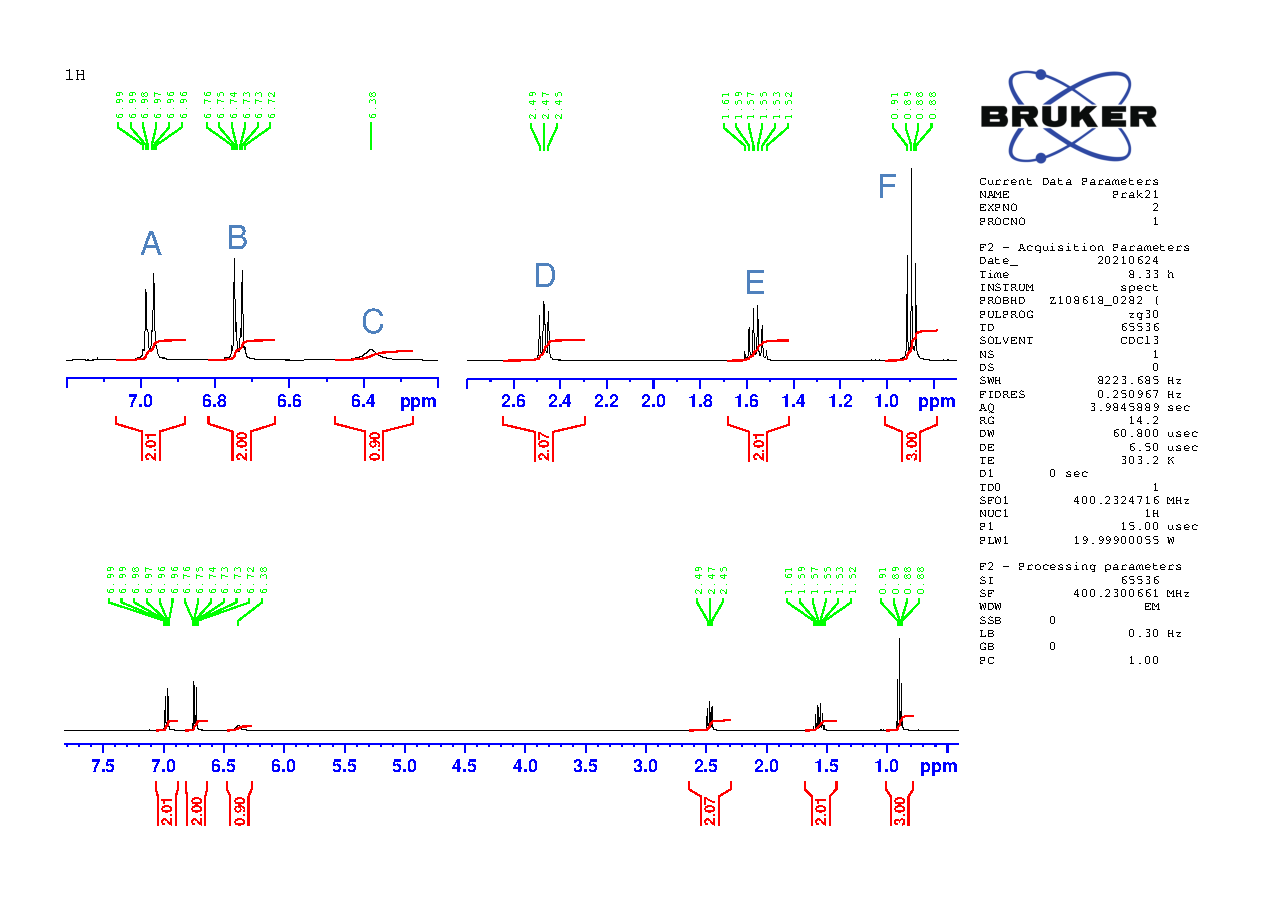
\includegraphics[page=1, width=\textwidth]{dokumente/spektrum_original.pdf}
		\caption{aufgenommenes ${}^1$H-NMR-Spektrum der unbekannten Probe}
		\label{fig:spektrum_original}
\end{figure}
\FloatBarrier


\section{Diskussion der Ergebnisse}
\label{sec:diskussion}

\subsection{Fragen der Praktikumsanleitung}
\begin{enumerate}
	\item \textit{Welche Kerne sind mit der NMR-Spektroskopie detektierbar?}\vspace*{1mm}\\
	Mit der NMR-Spektroskopie sind g/u-Kerne, u/g-Kerne und u/u-Kerne detektierbar. Der erste Buchstabe steht in dieser Angabe für die Anzahl der Protonen im Kern, der zweite Buchstabe für die Anzahl an Neutronen. Charakterisiert werden beide Zahlen mit \textit{u} und \textit{g}, was für eine gerade oder ungerade Anzahl des jeweiligen Kernbausteins steht. 
	\item \textit{Welche Größen spielen für die Empfindlichkeit der NMR-Spektroskopie eine Rolle?}\vspace*{1mm}\\
	Die Empfindlichkeit der NMR-Spektroskopie hängt von den folgenden Größen ab:
	\begin{itemize}
		\item Häufigkeit des Isotops
		\item Spinquantenzahl des betrachteten Isotops
		\item Unterschied der Energiezustände\\
		$\rightarrow$ proportional zur äußeren Magnetfeldstärke\\
		$\rightarrow$ proportional zum gyromagnetischen Verhältnis
		\item Temperatur
	\end{itemize}
	
	\item \textit{Bei welchem Auslenkungswinkel der Magnetisierung wird das größte Signal induziert? Wie wirkt sich eine Erhöhung der Senderleistung aus?}\vspace{1mm}\\
	Das größte Signal wird bei einem Drehwinkel der Magnetisierung von \SI{90}{\degrees} induziert. Je höher die Senderleistung ist und desto länger der Impuls der Senderspule andauert, desto weiter werden die Magnetisierungen der Probe gedreht und desto größer ist das induzierte Signal mit \SI{90}{\degrees} als Maximum.
	
	\item \textit{Durch welche Ursachen können magnetische Abschirmeffekte entstehen? Wie wird der Nullpunkt der Achse der chemischen Verschiebung festgelegt?}\vspace{1mm}\\
	Magnetische Abschirmeffekte können durch Einflüsse auf die Elektronenhülle des betrachteten Kerns entstehen. Diese können beispielsweise durch elektronenziehende Atome wie O, N oder Cl beeinflusst werden. Aber auch Doppel- und Dreifachbindungen, sowie Kreis- und Ringstromeffekte an Aromaten können eine derartige Abschirmung beeinflussen.\\
	Der Nullpunkt der Achse wird durch eine Referenzprobe festgelegt. Üblicherweise wird hierfür TMS (Tetramethylsilan) genutzt. Genutzt wird TMS, da es chemisch weitestgehend inert ist und dass es bei einer niedrigeren Frequenz als die gewöhnlichen organischen Verbindungen lediglich ein einziges, intensives Signal liefert. Grund hierfür ist, dass die Wasserstoffatome im TMS stark abgeschirmt sind und es fast keine weiteren Gruppen mit derart hoher Abschirmung gibt.
	\item \textit{Sie identifizieren in einem ${}^1$H-Spektrum ein Triplett bei \SI{0,9}{\ppm} mit einem Integralwert von 3. Welche Annahmen können Sie treffen?}
	\begin{itemize}
		\item Triplett: bedeutet es sind zwei benachbarte H-Atome am nächsten C-Atom, der untersuchten H-Atome \\
		$\rightarrow$ deutet auf eine angrenzende \ce{CH2}-Gruppe
		\item \SI{0,9}{\ppm}: lässt auf eine starke Abschirmung schließen \\
		$\rightarrow$  deutet darauf dass keine stark elektronegativen Gruppen an die Teilstruktur angrenzen
		\item Integralwert = 3: es werden drei gleichwertige H-Atome gemessen \\
		$\rightarrow$ deutet auf eine \ce{CH3}-Gruppe
		\end{itemize}
	\item \textit{Warum werden in der NMR-Spektroskopie deuterierte Lösungsmittel verwendet?}\vspace{1mm}\\
	Deuterierte Lösungsmittel haben den Vorteil, dass diese im ${}^1$H-NMR praktisch keine Lösungsmittelsignale erkennen lassen. Zu dem kann die Deuterium-Resonanz als Lock-Signal genutzt werden, um die Stabilität des Magnetfeldes zu überprüfen und Messparameter nachzukorrigieren.
\end{enumerate}

\newpage

\subsection{Auswertung des aufgenommenen Spektrums}
\subsubsection*{chemische Verschiebung}
Es wurden sechs Signale aufgenommen, was für sechs verschiedene Teilstrukturen in der gesuchten Verbindung stehen kann. In Abb. \ref{fig:spektrum_original} sind die einzelnen Signale mit den Buchstaben A bis F aufgeführt. 
Von A nach F verringert sich die chemische Verschiebung der jeweiligen Signale.
\vspace*{-2mm}
\subsubsection*{Kopplungsmuster}
Die Signale A und B weisen chemische Verschiebungen von \SI{6,98}{\ppm} und \SI{6,74}{\ppm} auf und weisen ein Multiplett höherer Ordnung auf. Diese Aspekte schließen auf eine aromatische Struktur. Zudem zeigt sich in dieser Struktur der sogenannte \textit{Dacheffekt}. Daraus lässt sich ableiten, dass sich in dieser aromatischen Struktur zweimal zwei chemische äquivalente Wasserstoffkerne befinden, welche nicht an das gleiche C-Atom gebunden sind. Es wird ein aromatischer Ring vermutet, welche zwei unterschiedliche Restgruppen in para-Stellung zueinander aufweist.\\
Das Signal C zeigt sich bei \SI{6,38}{\ppm} als schwaches breites Signal in Form eines Singuletts. Typisch für eine solche breite Verteilung eines Signals ist eine \ce{OH}-Gruppe, dessen Proton in Verbindungen als labil gilt. Dass das Signal ein Singulett ist deutet darauf hin, dass keine Spin-Spin-Kopplungen auftreten und daher keine Wasserstoffkerne in direkt benachbarten Teilstrukturen vorzufinden sind. Es wird vermutet, dass diese \ce{OH}-Gruppe eine der in para-Stellung stehenden Restgruppen ist. Demnach würde eine phenolische Struktur aus dem Spektrum hervorgehen.\\
Signal D weißt bei \SI{2,47}{\ppm} mit drei Peaks ein Triplett auf. Dies deutet darauf, dass die benachbarte Teilstruktur zwei Wasserstoffatome aufweist. Man könnte für diese benachbarte Struktur eine \ce{CH2}-Gruppe vermuten.\\
Signal E hingegen weißt bei \SI{1,56}{\ppm} mit sechs Peaks ein Sextett auf. Dies deutet darauf, dass die benachbarte Teilstruktur fünf Wasserstoffkerne aufweist. Ein solche Teilstruktur wäre mit einer \ce{CH3}- und einer \ce{CH2}-Gruppe gegeben. Mit \SI{1,56}{\ppm} ist diese Struktur stärker abgeschirmt als die Struktur bei Signal D. \\
Signal F weißt ausgehenden von der Anzahl der Signale, die durch den Computer bestimmt wurden bei \SI{0,89}{\ppm} ein Quartett auf. Augenscheinlich sind jedoch drei, statt vier Peks im Spektrum erkennbar und zwei der vom Computer ermittelten Peaks weisen die selbe chemische Verschiebung bei \SI{0,88}{\ppm} auf. Es wird daher davon gegangen, dass tatsächlich mit drei Peaks ein Triplett vorliegt. Ein solches Triplett deutet wiederum auf zwei benachbarte Wasserstoffkerne und somit auf eine \ce{CH2}-Gruppe. Mit \SI{0,88}{\ppm} ist diese Struktur stärker abgeschirmt als die Struktur bei Signal E.\\
Die Signale D, E und F deuten mit ihrer Struktur auf eine aliphatische Seitenkette als zweite Restgruppe an der aromatischen bzw. vielleicht phenolischen Verbindung.
\vspace*{-5mm}
\subsubsection*{Signalintensität}
Neben den Kopplungsmustern, der chemischen Verschiebung und der Anzahl der Signale sind auch die Signalintensitäten der einzelnen Signale ablesbar. Diese entsprechen der Anzahl der jeweils gemessenen Wasserstoffkerne des Moleküls.\\
Somit würde sich die Signale A und B mit Intensitäten von $2,01$ und $2,00$ in vier Wasserstoffatome an einem aromatischen Ring zusammenfassen. Dies deckt sich mit der Vermutung im Kopplungsmuster. \\
Signal C deutet mit einer Intensität von $0,90$ auf die \ce{OH}-Gruppe mit einem  einzigen Wasserstoffkern.\\
 Signal D spricht mit einer Intensität von $2,07$ für eine \ce{CH2}-Gruppe. Laut dem Kopplungsmuster würde sich an diese \ce{CH2}-Gruppe eine weitere \ce{CH2}-Gruppe anschließen.\\
 Signal E spricht mit einer Intensität von $2,01$ und demzufolge zwei Wasserstoffatomen, ebenfalls für eine \ce{CH2}-Gruppe. Laut Kopplungsmuster könnte diese \ce{CH2}-Gruppe an eine \ce{CH3}- und eine \ce{CH2}-Gruppe geknüpft sein.\\
 Signal F lassen sich mit einer Intensität von $3,00$, drei Wasserstoffkerne und somit eine \ce{CH3}-Gruppe zu ordnen. Diese \ce{CH3}-Gruppe ist entsprechend dem angepassten Kopplungsmuster mit einer weiteren \ce{CH2}-Gruppe benachbart.\\
 Bevorzugt aus den Intensitäten über die letzten drei Signale D bis F lässt sich nun ein Rückschluss daraus ziehen, dass definitiv eine aliphatische Kette als zweite Gruppe in para-Stellung zur \ce{OH}-Gruppe vorzufinden ist. Aus den Angaben der Intensitäten und der Kopplungsmuster lässt des Weiteren vermuten, dass diese zweite Gruppe ein Propyl-Rest ist. Das Partialspektrum einer solchen Propyl-Kette wird unter anderem in Quelle \cite[S. 17]{Breitmaier.2005} aufgeführt und gleicht sich mit dem aufgenommen Spektrum in Abb. \ref{fig:spektrum_original} bzw. der Signale D, E und F. 
 
 Als Folge der ausgeführten Aspekte die sich aus dem Spektrum ableiten lassen, führen demnach zu der in Abbildung \ref{fig:struktur_linear} dargestellten Struktur. Die Zuordnung der Messsignale erfolgt nach der jeweiligen Abschirmung der betrachteten Wasserstoffkerne in der Verbindung (siehe Abb. \ref{fig:struktur_linear}).
 
\begin{figure}[h!]
	\centering
	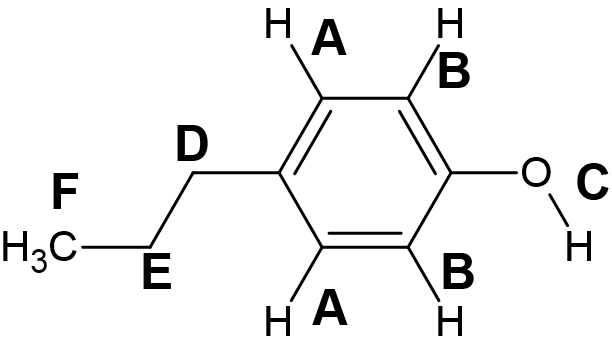
\includegraphics[width=0.33\textwidth]{img/struktur_linear_b.png}
	\caption{ermittelte Strukturformel (p-Propyphenol)}
	\label{fig:struktur_linear}
\end{figure}
\FloatBarrier

\subsection{Begründung der Probenstruktur}
Um weiter die Struktur in Abb. \ref{fig:struktur_linear} der unbekannten Probe begründen zu können, werden weitere Quellen hinzugezogen. In diesem Fall werden zwei recherchierte Spektren zum p-Propylphenol mit dem aufgenommenem Spektrum verglichen.
Zunächst wurde ein ${}^1$H-NMR-Spektrum mit Hilfe der Quelle \cite{Patiny.30.06.2021} simuliert. Auf der angegebenen Website lässt sich eine Struktur zeichnen oder Hochladen und infolgedessen ein Spektrum dazu simulieren. Zu beachten ist jedoch, dass auf der Website vermerkt ist, dass labile Protonen, wie in \ce{NH}-, \ce{CO2H}- oder \ce{OH-}Gruppen, nicht simuliert werden.
Das simulierte Spektrum ist in Abb. \ref{fig:spektrum_simuliert} zu sehen.
\begin{figure}[h!]
	\centering
	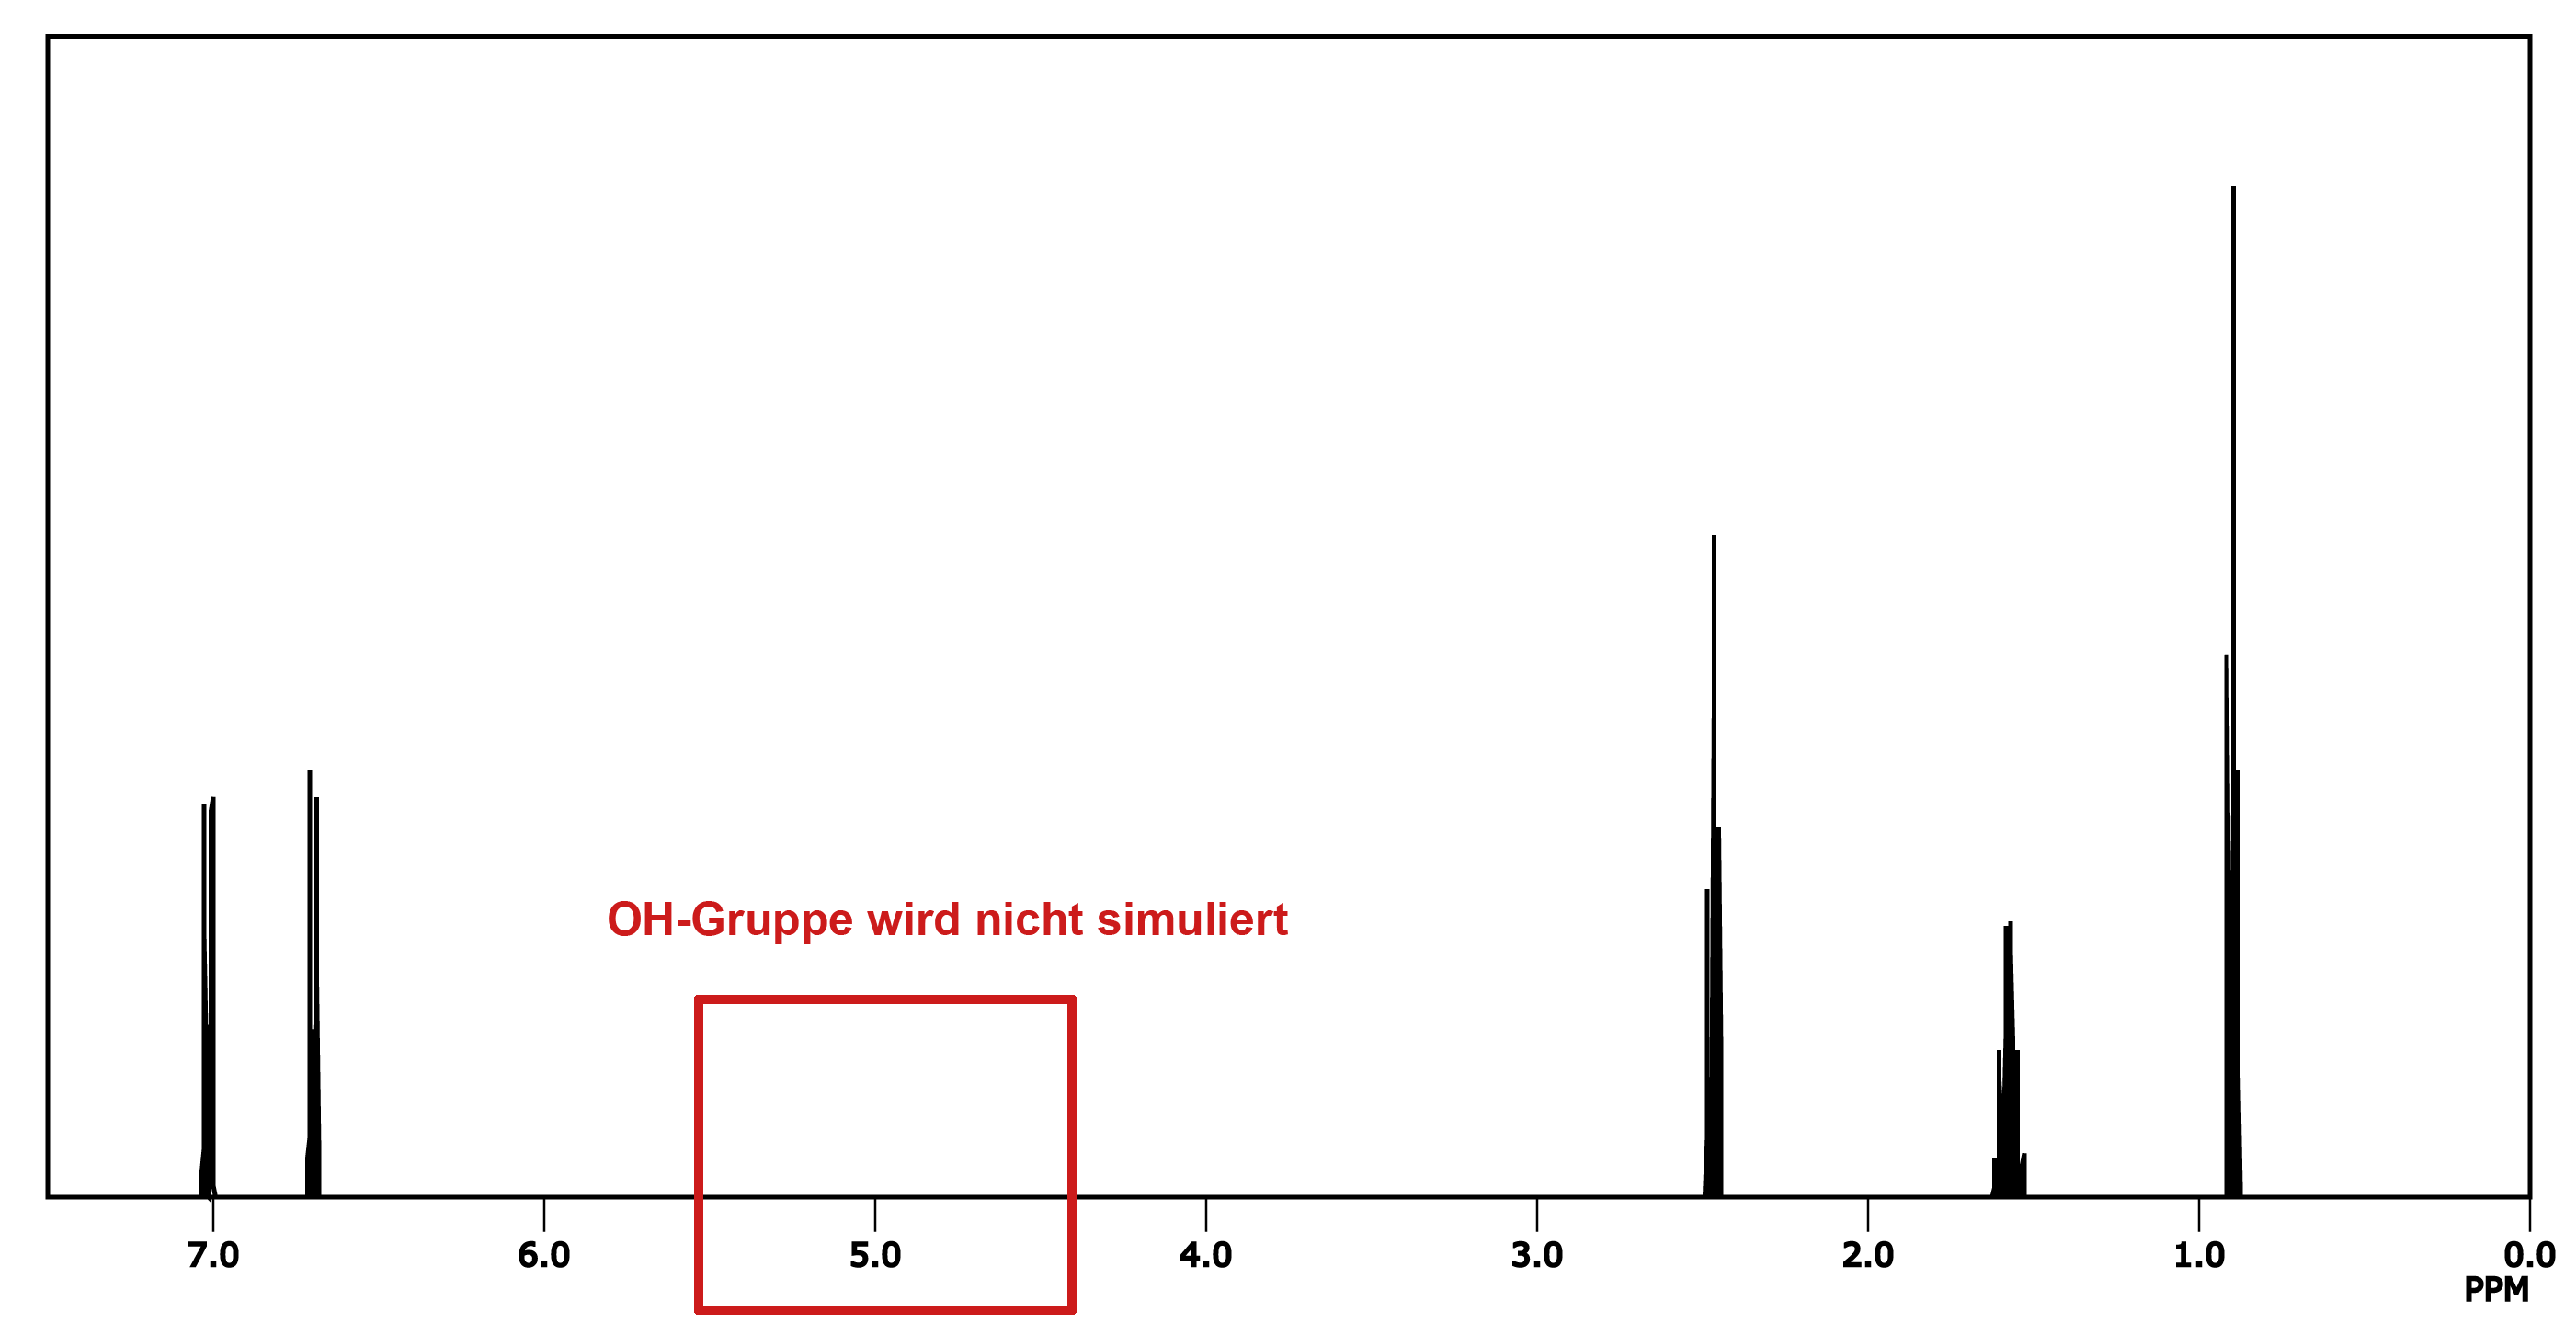
\includegraphics[width=\textwidth]{img/spektrum_simuliert_gesamt_oh.png}
	\caption{mit \url{www.nmrdb.org} simuliertes Spektrum von p-Propylphenol \cite{Patiny.30.06.2021}}
	\label{fig:spektrum_simuliert}
\end{figure}

Vergleicht man das simulierte Spektrum in Abb. \ref{fig:spektrum_simuliert} mit dem aufgenommen Spektrum in Abb. \ref{fig:spektrum_original} fällt auf, dass diese Spektren sich sehr ähnlich sind in Bezug auf die vorliegenden Kopplungsmuster. Weiterhin sind lediglich geringe Abweichungen in den chemischen Verschiebungen der Signale festzustellen. In der Anzahl der Messsignale unterscheiden sich jedoch beide Spektren, das die \ce{OH}-Gruppe des p-Propylphenols, wie zuvor beschrieben, nicht mit simuliert wird.
Lässt man den fehlenden \ce{OH}-Peak außer Acht begründetet das simuliert Spektrum bereits die bestimmte Struktur der Probe. 
\newpage
Weiterhin wird die Annahme, dass Peak F im originalen Spektrum ein Triplett ist, durch das simulierte Spektrum augenscheinlich bestätigt.\\
Um nicht nur ein simuliertes Spektrum als Rechtfertigung für die bestimmte Struktur in Abb. \ref{fig:struktur_linear} vorweisen zu können, wird zusätzlich eine Spektrendatenbank genutzt. In dieser wird konkret nach der bestimmten Struktur und dessen ${}^1$H-NMR-Spektrum gesucht. Vorteil einer solchen Datenbank ist es, dass die Verbindungen nicht simuliert, sondern real vermessen wurden. Die zu erwartenden Spektren sind demnach mit dem im Praktikum aufgenommen Spektrum besser zu vergleichen. Als NMR-Datenbank wurde die \textit{Spectral Database for Organic Compounds} alias \textit{SDBS} genutzt \cite{AIST.30.06.2021}. Das dort gefundene Spektrum für p-Propylphenol ist in Abbildung \ref{fig:spektrum_sdbs} dargestellt.

\begin{figure}[h!]
	\centering
	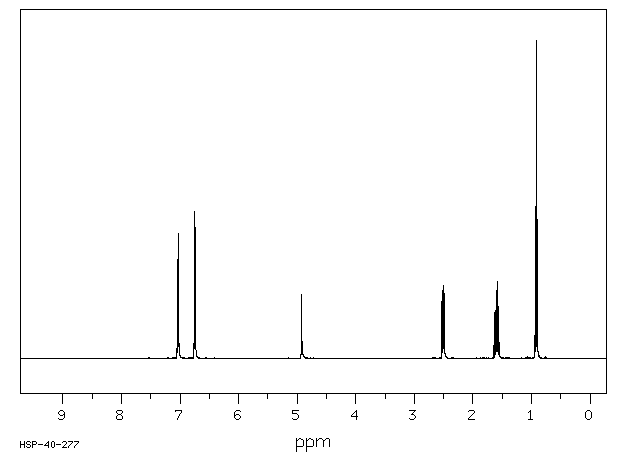
\includegraphics[width=0.75\textwidth]{img/sdbs_spektrum.png}
	\caption{Spektrum von p-Propylphenol aus der \textsc{AIST} SDBS-Datenbank \cite{AIST.30.06.2021}}
	\label{fig:spektrum_sdbs}
\end{figure}
\FloatBarrier

Auch in diesem Spektrum erscheinen die chemische Verschiebung, sowie das Kopplungsmuster sehr ähnlich zum selbst gemessenen Spektrum. Zudem fällt auf, dass im Vergleich zum simulierten Spektrum in Abb. \ref{fig:spektrum_simuliert} auch ein Peak für die  \ce{OH}-Gruppe zu verzeichnen ist. Mögliche Unterschiede könnten sich durch Signalrauschen oder leicht unterschiedliche Messbedingungen erklären lassen. Weiterhin ist auch in diesem Spektrum das äußerste Signal mit der kleinsten chemischen Verschiebung als Triplett zu charakterisieren.
Somit untermauert das Vergleichsspektrum für p-Propylphenol ebenfalls die bestimmte Struktur in Abb. \ref{fig:struktur_linear} des aufgenommenen Spektrums in \mbox{Abb. \ref{fig:spektrum_original}}. \\

Für die unbekannte Probe wird daher behauptet, dass es sich um die organische Verbindung p-Propylphenol alias 4-Propylphenol handelt.

%\section{Zusammenfassung und Fazit}
\label{sec:zusammenfassung}


%\section{Fehlerbetrachtung}
\label{sec:fehler}


%%Praktikumsskript, Modul ………, Versuch …….., Prof. Musterprof. 
%%DIN 12345, Jahr der Veröffentlichung 
%%Link der Internetseite, Zugriffsdatum 
%%Buchtitel, Autor, Verlag, Veröffentlichungsjahr 
%
%Literaturverzeichnis Bücher

\vfill
\bibliography{Literatur}
\bibliographystyle{unsrtdin}
\addcontentsline{toc}{section}{Literaturverzeichnis}



%\section*{Anhang}
\addcontentsline{toc}{section}{Anhang}
\label{sec:anhang}

%Betriebsanweisung

%\chapter*{Eidesstattliche Erklärung}
\label{erklaerung}
Hiermit versichere ich, die vorliegende Seminararbeit selbstständig und nur unter Verwendung der von mir angegebenen Quellen und Hilfsmittel verfasst zu haben. Sowohl inhaltlich als auch wörtlich entnommene Inhalte wurden als solche kenntlich gemacht. Die Arbeit hat in dieser oder vergleichbarer Form noch keinem anderem Prüfungsgremium vorgelegen. \\
\\[1.5cm]
Datum:	\hrulefill\enspace Unterschrift: \hrulefill
\\[3.5cm]
\addcontentsline{toc}{chapter}{Selbstständigkeitserklärung}

\end{document}
